\documentclass[tikz,border=4pt]{standalone}
\usepackage{amsmath,amssymb}
\usetikzlibrary{arrows.meta,calc,decorations.pathreplacing}
\definecolor{cA}{HTML}{924800}
\definecolor{cB}{HTML}{2F7FC8}
\definecolor{cC}{HTML}{39994B}
\tikzset{
  pt/.style={circle,fill=black,inner sep=0pt,minimum size=4pt},
  disp/.style={-{Stealth[length=2.6mm,width=2mm]},line width=0.9pt,shorten <=2.5pt,shorten >=2.5pt},
  lab/.style={font=\small,sloped,text=black},
  brc/.style={decorate,decoration={brace,amplitude=5pt,raise=3pt},line width=0.6pt},
}
\begin{document}
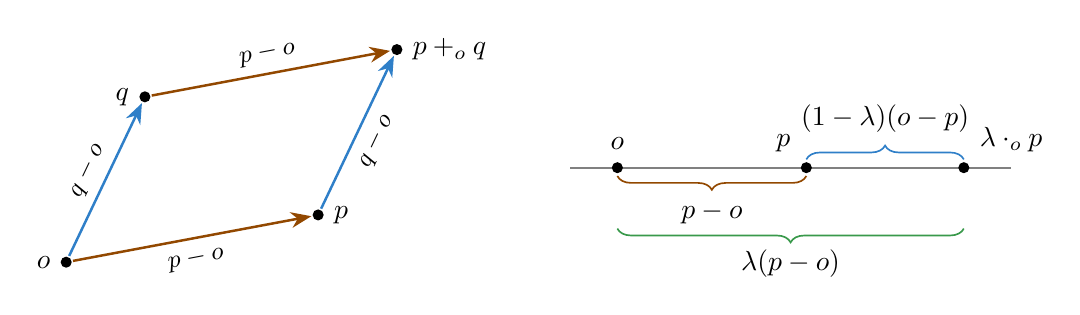
\begin{tikzpicture}
  % addition
  \coordinate (o) at (0,0); \coordinate (p) at (3.2,0.6); \coordinate (q) at (1.0,2.1);
  \coordinate (pq) at ($(p)+(q)-(o)$);
  \draw[disp,cA] (o) -- node[lab,below]{$p-o$} (p);
  \draw[disp,cA] (q) -- node[lab,above]{$p-o$} (pq);
  \draw[disp,cB] (o) -- node[lab,above]{$q-o$} (q);
  \draw[disp,cB] (p) -- node[lab,below]{$q-o$} (pq);
  \node[pt,label=left:$o$] at (o) {}; \node[pt,label=right:$p$] at (p) {};
  \node[pt,label=left:$q$] at (q) {}; \node[pt,label=right:$p+_o q$] at (pq) {};
  % scalar multiplication
  \begin{scope}[xshift=7cm,yshift=1.2cm]
    \coordinate (o) at (0,0); \coordinate (p) at (2.4,0); \coordinate (lp) at (4.4,0);
    \draw[gray,line width=0.6pt] (-0.6,0) -- (5.0,0);
    \draw[brc,cA] (p) -- node[below=9pt,text=black]{$p-o$} (o);
    \draw[brc,cC,decoration={raise=22pt}] (lp) -- node[below=26pt,text=black]{$\lambda(p-o)$} (o);
    \draw[brc,cB] (p) -- node[above=9pt,text=black]{$(1-\lambda)(o-p)$} (lp);
    \node[pt,label={[label distance=1pt]above:$o$}] at (o) {};
    \node[pt,label={[label distance=1pt]above left:$p$}] at (p) {};
    \node[pt,label={[label distance=1pt]above right:$\lambda\cdot_o p$}] at (lp) {};
  \end{scope}
\end{tikzpicture}
\end{document}
